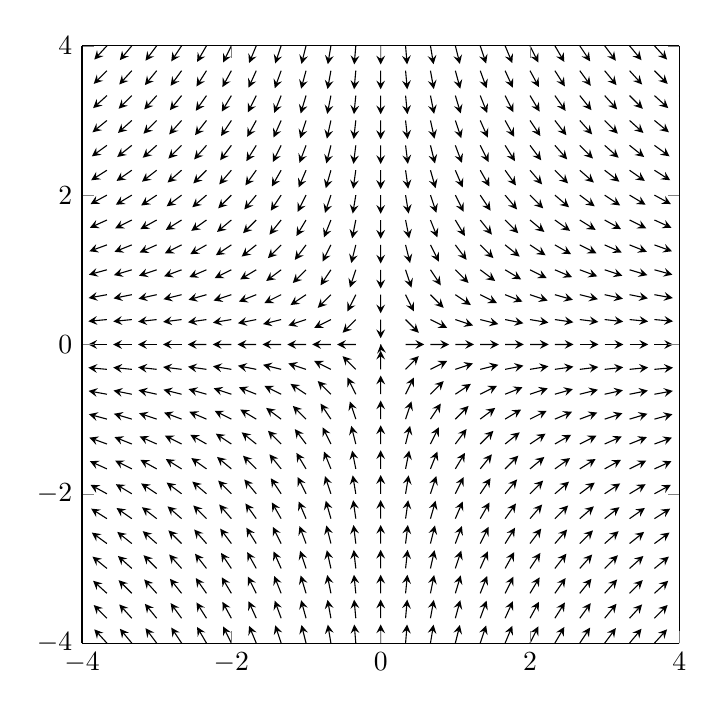
\begin{tikzpicture}
        \begin{axis}[
            xmin = -4, xmax = 4,
            ymin = -4, ymax = 4,
            zmin = 0, zmax = 1,
            axis equal image,
            xtick distance = 2,
            ytick distance = 2,
            view = {0}{90},
            scale = 1.4,
            height=7cm,
            %xlabel = {$x$},
            %ylabel = {$y$}
        ]
            \addplot3[
                point meta = {sqrt(x^2+y^2)},
                quiver = {
                    u = {x/sqrt(x^2+y^2+0.0001)},
                    v = {-y/sqrt(x^2+y^2+0.000001)},
                    scale arrows = 0.25,
                },
                %quiver/colored = {mapped color},
                -stealth,
                domain = -4:4,
                domain y = -4:4,
            ] {0};
        \end{axis}
    \end{tikzpicture}\\